\documentclass{article}

\ifdefined\HCode
\def\pgfsysdriver{pgfsys-tex4ht.def}
\fi
\usepackage{tikz}
\usepackage{tikz-cd}

\begin{document}
  Test!

  \begin{equation}\label{eq:nat_vertical}
    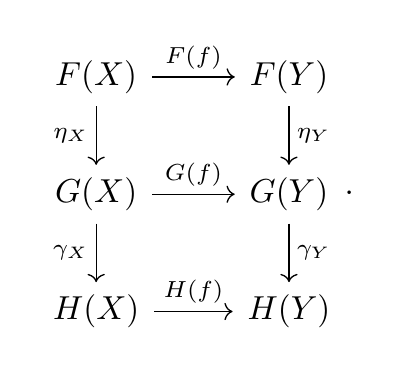
\begin{tikzpicture}[baseline= (a).base]
      \node[scale=1.2] (a) at (0,0) {
        \begin{tikzcd}
          F (X) \arrow[r, "F (f)"] \arrow[d, "\eta_{X}"']
          &  F (Y) \arrow[d, "\eta_{Y}"]
          \\ G (X) \arrow[r, "G (f)"] \arrow[d, "\gamma_{X}"']
          &  G (Y) \arrow[d, "\gamma_{Y}"]
          \\ H (X) \arrow[r, "H (f)"]
          &  H (Y)
        \end{tikzcd}.
      };
    \end{tikzpicture}
  \end{equation}
\end{document}
